\documentclass[a4paper,UTF8]{ctexart}

\usepackage{amsmath, amsthm, amssymb, amsfonts, hyperref, mathrsfs}%美国数学学会的包+?
\usepackage{geometry} %控制界面
\usepackage{bookmark}
\usepackage{fancyhdr} % header & footer
\usepackage{appendix} % 附录
\usepackage{tikz} %作图
\usepackage{graphicx} %插入图片的宏包
\usepackage{float} %设置图片浮动位置的宏包
\usepackage{subfigure} %插入多图时用子图显示的宏包
\usepackage{listings} %引用代码
\usepackage{physics,mathtools} %物理数学工具
\geometry{top=2.5cm,bottom=2.5cm,left=2.5cm,right=2.5cm} % 布局要求
\pagestyle{fancy} % fancy分格
\fancyhf{} % 清除所有页眉页脚
\renewcommand\headrulewidth{0.6pt}
\renewcommand\footrulewidth{0.6pt}
\lhead{何金铭 PB21020660}
\chead{座位号:4}
\rhead{\thepage}
\lfoot{2022.10.14}
\rfoot{USTC}
\bibliographystyle{plain} % 引用样式
\everymath{\displaystyle} % display
%============================================================

\begin{document}

\begin{center}
    \textbf{\Large 偏振光的研究}
    \par \text{\large 何金铭 PB21020660}
\end{center}

\section{实验目的}
研究偏振光的若干性质
\section{实验原理}

\subsection{产生偏振光的元件}

\subsubsection{利用光在界面反射和透射时光的偏振现象}

利用光的电磁理论可以计算出光于不同方向的偏振改变,反射光中的垂直于入射面的光振动(称 s 分量)多于平行于入射面的光振动(称 p 分量);而透
射光则正好相反。当入射角为布儒斯特角$i_b$时,反射光为完全线偏振光(s分量)。
此时有:

\begin{equation*}
    i_b+\gamma_0 = \frac{\pi}{2} \  , \ n_1 \sin{i_b} = n_2 \sin{\gamma_0} 
\end{equation*}

\begin{equation*}
    \tan{i_b} = \frac{\sin{i_b}}{\cos{i_b}} = \frac{\sin{i_b}}{\sin{\gamma_0}} = \frac{n_2}{n_1}
\end{equation*}

$n_1 = 1$(空气折射率)时,有

\begin{equation}
   n_2 = \tan{i_b} 
\end{equation}

所以通过测量布儒斯特角的大小可以测量介质的折射率。

\subsubsection{利用光学棱镜——双折射现象}

利用某些特定晶体的双折射现象可制备格兰棱镜,其由两块方解石直角棱镜构成,两棱镜间有空气间隙,方解石的光轴平行于棱镜的棱。
自然光垂直于界面射入棱镜后分为 o 光和 e 光,o 光在空气隙上全反射,只有 e 光透过棱镜射出。

\subsubsection{偏振片}

它是利用聚乙烯醇塑胶膜制成,它具有梳状长链形结构分子,这些分子平行
排列在同一方向上,此时胶膜只允许垂直于排列方向的光振动通过,因而产生线偏振光。

\subsection{改变光的偏振态的元件——波晶片}

波晶片又称相位延迟片。它是从单轴晶体中切割下来的平行平面板(其光轴方向与表面平行),
由于波晶片内 o 光和 e 光的传播速度 $v_o$ 、$v_e$ 不同(折射率 $n_o$、$n_e$ 不同),所以造成 o 光和 e 光通
过波晶片的光程也不同。由此产生了相位的变化。

比如$\lambda / 4$波片可以用来改变光的偏振态,改变相位为$\frac{\pi}{2}$

\section{实验仪器}
半导体激光器(波长 650 nm)、 硅光电池、 起偏器、 检偏器、 旋转样品台、 数字式检流计


\section{实验内容}

\begin{enumerate}
    \item 仪器调节
    \item 测量半导体激光器的偏振度
    \item 验证马吕斯定律
    \item 利用已给实验仪器,根据布儒斯特定律,自行设计实验方案测定玻璃介质的折射率。
    \item 利用已给实验仪器(偏振片、1/4 波片),判断液晶屏(手机屏、大屏显示器等)所发出光线
的偏振状态(线偏振、圆偏振、自然光等)。给出判断结果及详细的判断过程。
\end{enumerate}

\section{测量记录}

\subsection{半导体激光器的偏振度}

\begin{table}[htb]
\begin{center}
\begin{tabular}{|c|c|c|c|}
\hline
\bfseries 光强极大值$(10^{-7}A)$ & \bfseries 偏振片角度$(^{\circ})$ & \bfseries 光强极小值$(10^{-7}A)$ & \bfseries 偏振片角度$(^{\circ})$\\
\hline
960                  & 246                  & 2                    & 333                  \\
\hline
943                  & 64                   & 2                    & 154                \\
\hline
\end{tabular}
\end{center}
\caption{光强1对应的数据}
\end{table}

\begin{table}[htb]
\begin{center}
\begin{tabular}{|c|c|c|c|}
\hline
\bfseries 光强极大值$(10^{-7}A)$ & \bfseries 偏振片角度$(^{\circ})$ & \bfseries 光强极小值$(10^{-7}A)$ & \bfseries 偏振片角度$(^{\circ})$\\
\hline
1729                  & 245                  & 4                    & 334                  \\
\hline
1694                  & 64                   & 4                    & 154                \\
\hline
\end{tabular}
\end{center}
\caption{光强2对应的数据}
\end{table}

\subsection{验证马吕斯定律}

\newpage

\begin{table}[htb]
\begin{tabular}{|c|c|c|c|}
\hline
\bfseries 透振方向夹角($\theta$ / $^\circ$) & \bfseries 透射光强($I$ / $(10^{-7}A)$) & \bfseries 透振方向夹角($\theta$ / $^\circ$) & \bfseries 透射光强($I$ / $(10^{-7}A)$) \\ \hline
84  & 0   & 132 & 483 \\ \hline
90  & 13  & 138 & 568 \\ \hline
96  & 44  & 144 & 648 \\ \hline
102 & 91  & 150 & 718 \\ \hline
108 & 154 & 156 & 775 \\ \hline
114 & 226 & 162 & 818 \\ \hline
120 & 308 & 168 & 844 \\ \hline
126 & 395 & 174 & 853 \\ \hline

\bfseries 透振方向夹角($\theta$ / $^\circ$) & \bfseries 透射光强($I$ / $(10^{-7}A)$) & \bfseries 透振方向夹角($\theta$ / $^\circ$) & \bfseries 透射光强($I$ / $(10^{-7}A)$) \\ \hline

180 & 844 & 228 & 297 \\ \hline
186 & 817 & 234 & 216 \\ \hline
192 & 772 & 240 & 146 \\ \hline
198 & 713 & 246 & 85  \\ \hline
204 & 642 & 252 & 39  \\ \hline
210 & 561 & 258 & 10  \\ \hline
216 & 475 & 264 & 0   \\ \hline
222 & 385 & 270 & 8   \\ \hline
\end{tabular}
\caption{透射光强与透振方向夹角记录表}
\end{table}

\subsection{测量样品布儒斯特角}

\subsubsection{方案一}

调节偏振片,使得偏振光的方向只有与入射面平行的分量。
从一个方向转动旋转样品台,起始位置为入射角为0的状态。
记录此时的刻度为$\alpha_i$
转动样品台,当出现反射光光强为0,或者接近0的状态时,
则说明此时转过的角度$\alpha = i_b$,为布儒斯特角。
记录此时的可得为$\alpha_f$

\subsubsection{方案二}
调节偏振片,使得偏振光的方向只有与入射面平行的分量。
从一个方向转动旋转样品台,起始位置为入射角为0的状态。
记录此时的刻度为$\alpha_1$
转动样品台,当出现反射光光强为0,或者接近0的状态时,
则说明此时转过的角度$\alpha = i_b$,为布儒斯特角。
接着继续旋转样品台,当发现反射光第二次为0的时候,
记录刻度$\alpha_2$,

\begin{figure}[H]
    \centering
    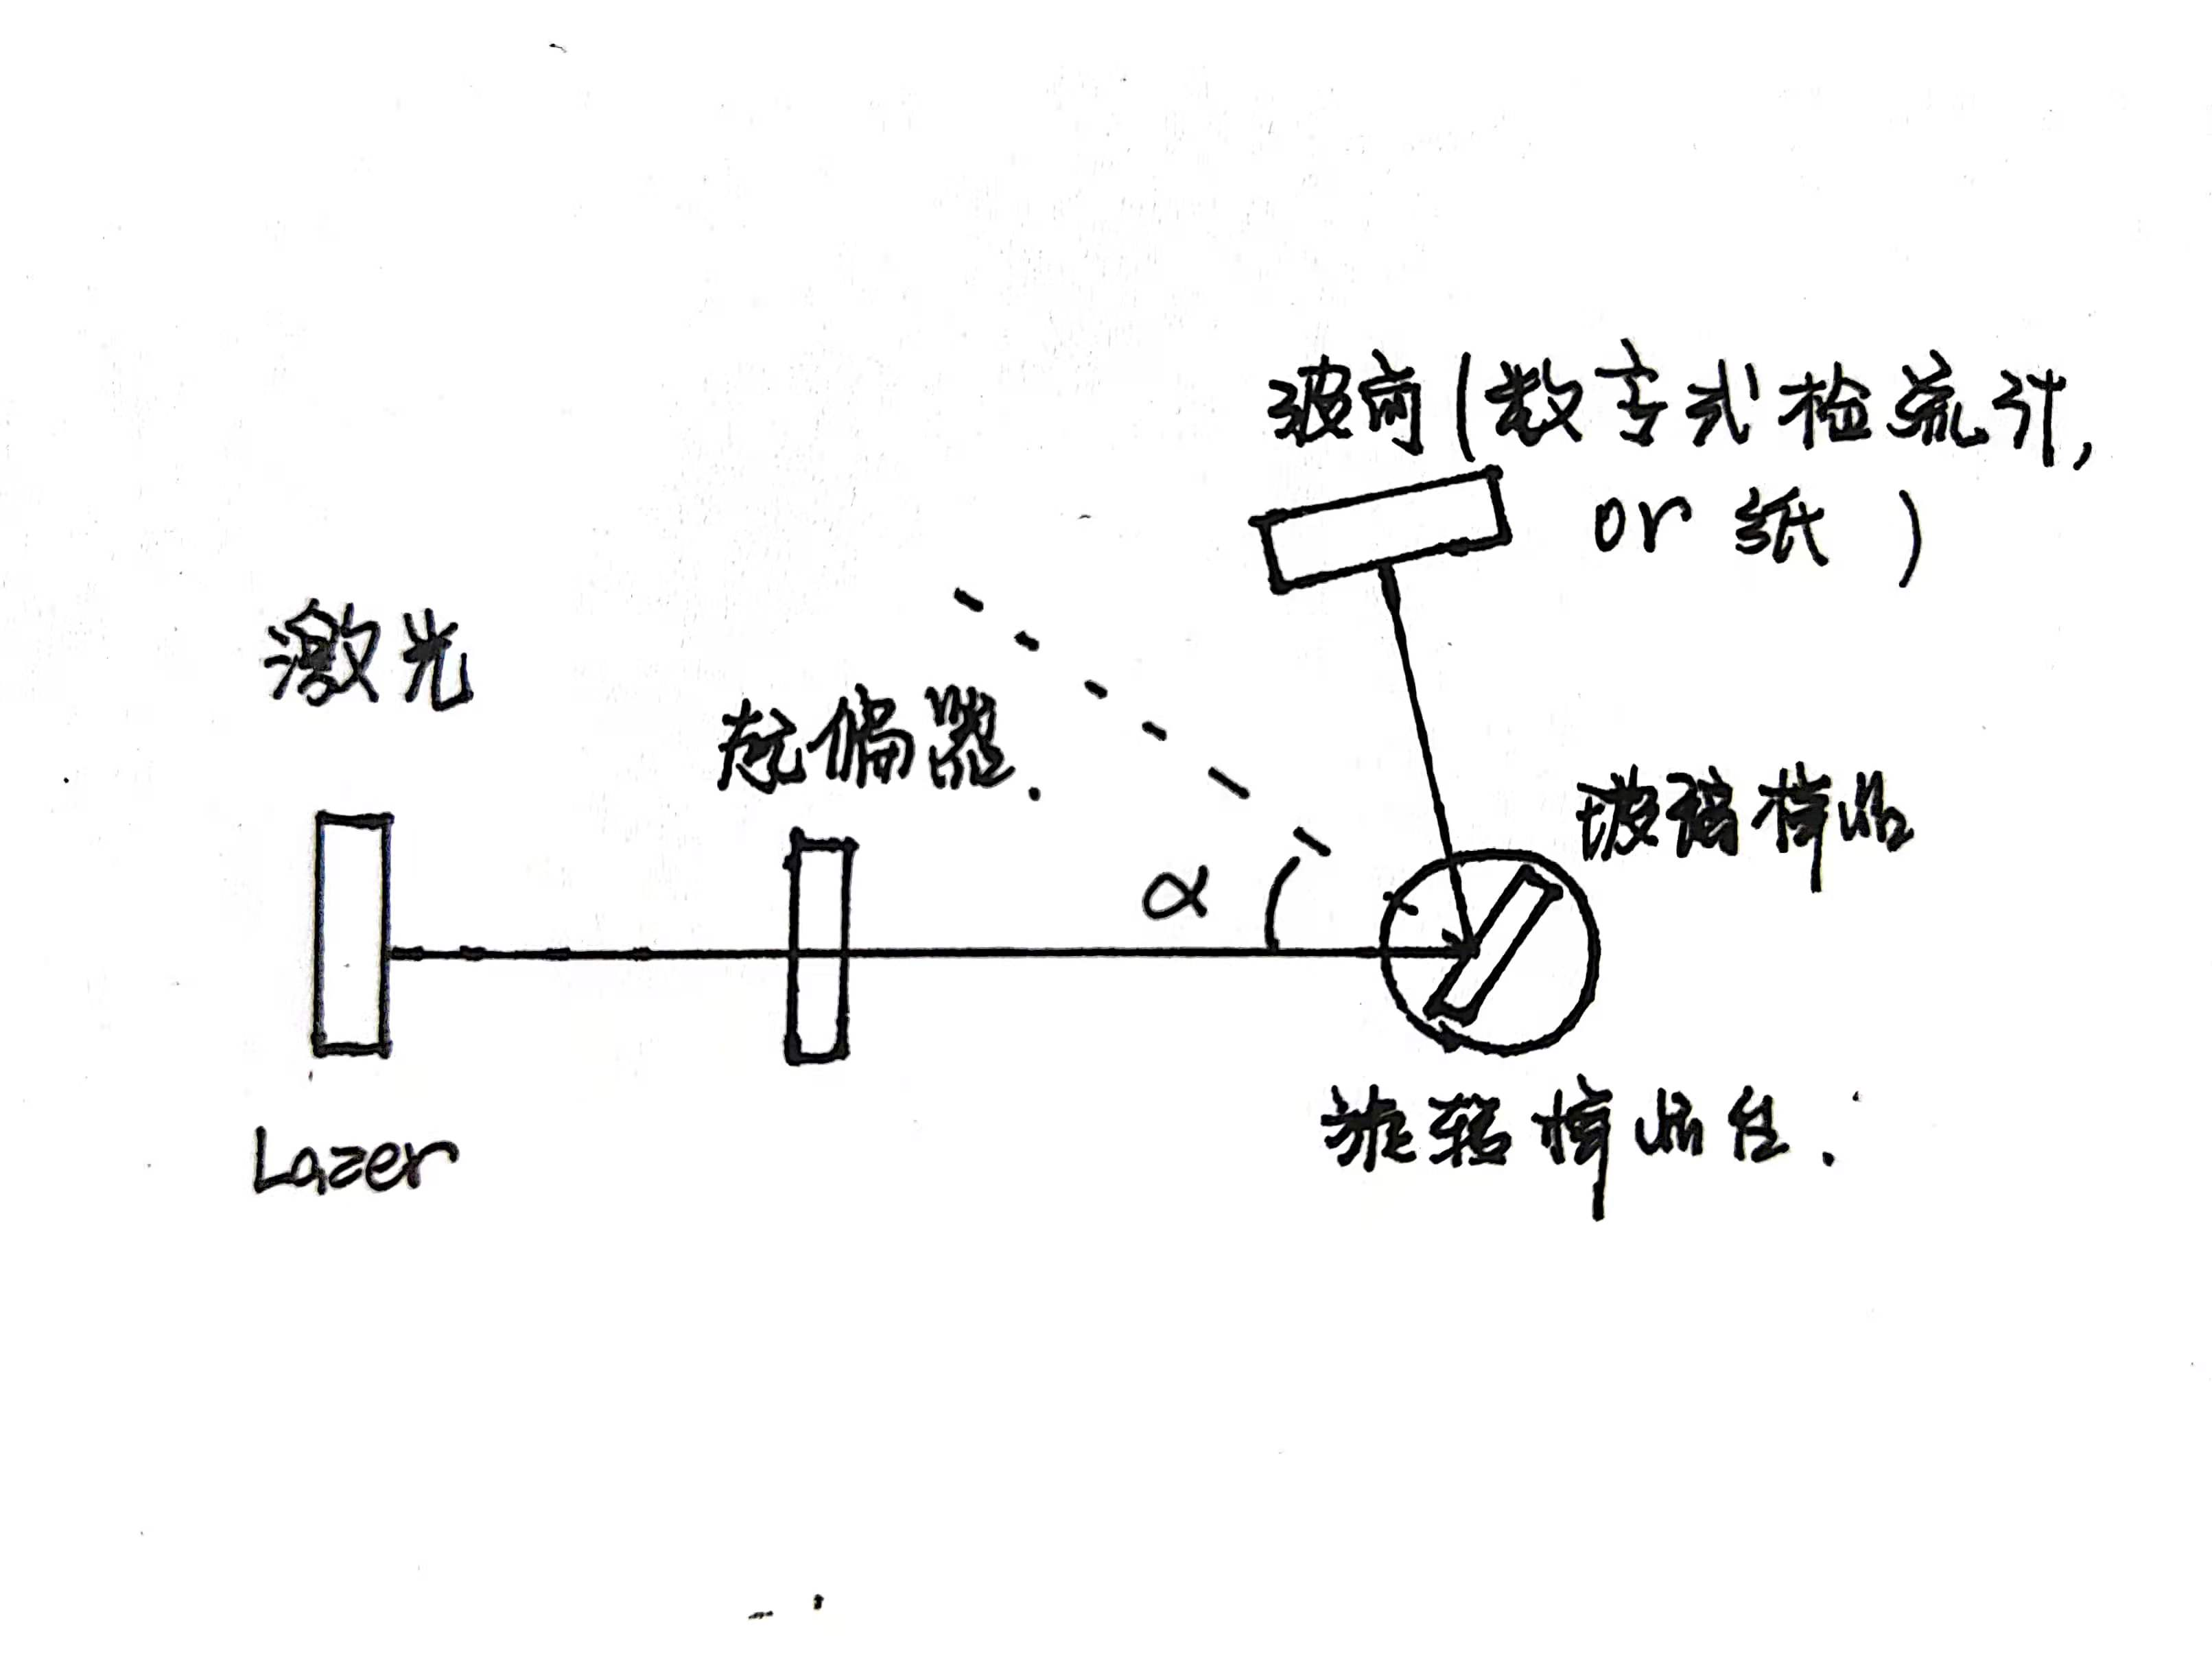
\includegraphics[width=0.8\textwidth]{1.jpg}
    \caption{实验光路图}
\end{figure}
\begin{table}[htb]
    \begin{center}
        \begin{tabular}{|c|c|c|}
            \hline
            & \bfseries 1 & \bfseries 2 \\
            \hline
            \bfseries $\alpha_{i}$ & $275.2 ^\circ$ & $21.0 ^\circ$   \\
            \hline
            \bfseries $\alpha_{f}$ & $217.0^\circ$ & $325.0^\circ$ \\
            \hline
        \end{tabular}
    \end{center}
    \caption{改进方案前的实验数据}
\end{table}

\begin{table}[htb]
    \begin{center}
        \begin{tabular}{|c|c|c|c|}
            \hline
            & \bfseries 1 & \bfseries 2 & \bfseries 3 \\
            \hline
            \bfseries $\alpha_1$ & $80.2 ^\circ$ & $80.0 ^\circ$ & $79.0 ^\circ$ \\
            \hline
            \bfseries $\alpha_2$ & $327.9^\circ$ & $327.2 ^\circ$ & $326.0 ^\circ$ \\
            \hline
        \end{tabular}
    \end{center}
    \caption{改进方案后的实验数据}
\end{table}

\subsection{判断教室大屏幕显示器所发出光线的偏振状态}

实验现象:通过一个偏振片看教室大屏幕,发现当改变偏振片偏振方向的时候可以发现
会出现明暗交替的现象,且会出现完全消光的现象。(事实上,是大面积的消光现象,如果仔细观察,还可以
看到一些斜着的明条纹,但是占少数。)

\section{分析与讨论}

\subsection{半导体激光器的偏振度}

\subsubsection{结果分析}

首先对数据进行分析,发现每次大约转动$90^\circ$时,激光的光强就会由最大值变为最小值。

由于光的最小光强不为0,所以得出激光器不是完美的线偏振光,而是一个椭圆偏振光,存在偏振度$P = \frac{I_{max}-I_{min}}{I_{max}+I_{min}}$。

由第一组数据可得:

\begin{equation}
    P_1 = \frac{I_{max}-I_{min}}{I_{max}+I_{min}} = \frac{\frac{960+943}{2}-2}{\frac{960+943}{2}+2}=0.9958
\end{equation}

\begin{equation}
    P_2 = \frac{I_{max}-I_{min}}{I_{max}+I_{min}} = \frac{\frac{1729+1694}{2}-4}{\frac{1729+1694}{2}+4}=0.9953
\end{equation}

发现两组数据测出来相似,偏振度的大约为$0.9955$,是一个理想的线偏振光。

\subsubsection{误差分析}

两组数据有一定偏差,其来源可能有:

\begin{enumerate}
    \item 测量时的误差导致
    \item 前后测量时,改变了数字式检流计的灵敏度,导致测量的偏振度发生了改变。
\end{enumerate}

\subsection{验证马吕斯定律}

定义透射光强$I=I_{max}=I_0$时的透振方向夹角$\theta = 0$,则变换上方数据中的数据$\theta' = \theta - 174^\circ$
变换后得到的$\theta' \in \left[-90^\circ,90^\circ\right]$

分别作图,得:

\begin{figure}[H]
    \centering
    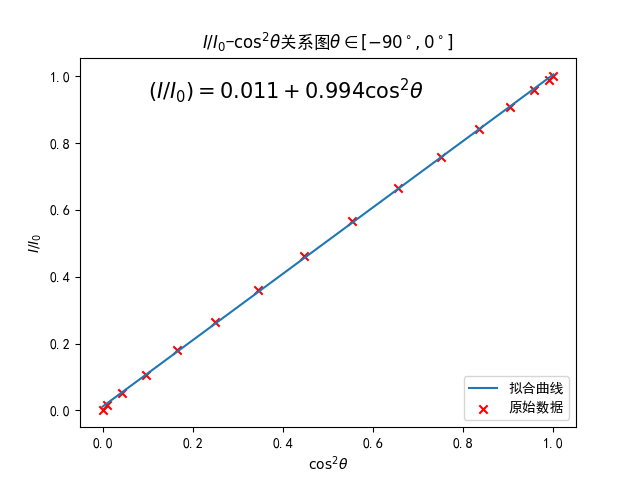
\includegraphics[width=0.8\textwidth]{n.png}
    \caption{$\frac{I}{I_0}$-$\cos^2{\theta}$关系图$\theta \in \left[-90^\circ,0^\circ\right]$}
\end{figure}

\begin{figure}[H]
    \centering
    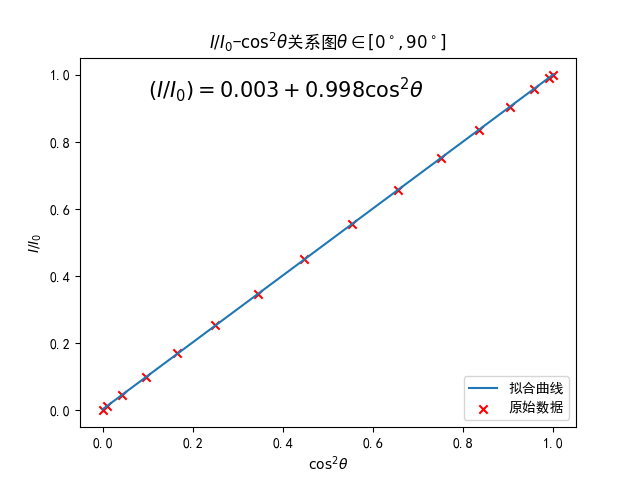
\includegraphics[width=0.8\textwidth]{p.png}
    \caption{$\frac{I}{I_0}$-$\cos^2{\theta}$关系图$\theta \in \left[0^\circ,90^\circ\right]$}
\end{figure}

并且利用最小二乘法给出了:

\begin{equation}
    \frac{I}{I_0} = \left\{
        \begin{array}{clr}
            0.011 + 0.994 \cos^2{\theta} & & \theta \in \left[-90^\circ,0^\circ\right] \\
            0.003 + 0.998 \cos^2{\theta} & & \theta \in \left[0^\circ,90^\circ\right] 
        \end{array}\right.
\end{equation}

$\theta \in \left[-90^\circ,0^\circ\right]$时,斜率为$0.994$,截距为$0.011$

$\theta \in \left[0^\circ,90^\circ\right]$时,斜率为$0.998$,截距为$0.003$

发现第二组的测量结果比第一组的测量结果更加接近理论值。但是两组的结果都在一定置信区间内符合要求“斜率为1,截距为0”

\subsubsection{误差分析}

误差来源有以下可能

\begin{enumerate}
    \item 前$90^\circ$与后$90^\circ$的误差不同,可能的原因是偏振片于两个$\frac{1}{4}$圆周上存在一定不对称结构。
    \item 由于光路是手动调节的,可能存在主面与光轴不垂直或光学主面间存在微小夹角。
    \item 数字式检流计的固有误差所导致的测量误差。
\end{enumerate}

\subsection{测量样品布儒斯特角}


\subsubsection{改进前的方案}

从一个方向转动,得布儒斯特角

\begin{table}[htb]
    \begin{center}
        \begin{tabular}{|c|c|c|c|}
            \hline
            & \bfseries 1 & \bfseries 2 & \bfseries average \\
            \hline
            \bfseries $i_b$ & $58.2^\circ$ & $56^\circ$ & $57.1^\circ$ \\
            \hline
        \end{tabular}
    \end{center}
    \caption{方案一结果}
\end{table}

由于方案一还存在着旋转样品台本身的误差,所以在这里只参考,不进行误差分析。

\subsubsection{改进后的方案}

利用$2i_b = \frac{360^\circ+\alpha_1-\alpha_2}{2}$得:

\begin{table}[htb]
    \begin{center}
        \begin{tabular}{|c|c|c|c|c|}
            \hline
            & \bfseries 1 & \bfseries 2 & \bfseries 3 & \bfseries average \\
            \hline
            \bfseries $i_b$ & $56.15^\circ$ & $56.4^\circ$ & $56.5^\circ$ & $56.35^\circ$\\
            \hline
        \end{tabular}
    \end{center}
    \caption{方案二结果}
\end{table}

\subsubsection{误差分析}

下面进行不确定度分析:

A类标准不确定度$u_A = \sqrt{\frac{\sum_{i=1}^{n} (X_i - \overline{X})^2}{n(n-1)}} = 0.1^\circ$

B类标准不确定度$u_B = \frac{\sqrt{\Delta_{app}^2+\Delta_{est}^2}}{C}=\frac{\sqrt{0.5^2+1^2}}{3}=0.37^\circ$

拓展不确定度$U_{i_b} = t_p u_A + k_p u_B = 1.2^\circ$

得布儒斯特角$i_b = 56.4^\circ \pm 1.2^\circ$

得玻璃的折射率为$n = \tan{i_b} = 1.51$

不确定度$U_n = \frac{1}{\cos{i_b}^2} U_{i_b} = 3.26 \cdot 1.2 \cdot \frac{\pi}{180} = 0.07$

最终得玻璃的折射率为$n = 1.51 \pm 0.07$

\begin{enumerate}
    \item 最终相对不确定度为$4\%$符合要求
    \item 误差可能来自于寻找偏振光为0时,手动寻找布儒斯特角的位置。
\end{enumerate}

\subsection{判断教室大屏幕显示器所发出光线的偏振状态}

大屏幕显示所发出的光绝大部分是线偏振光。

实验操作时通过一个偏振片看教室大屏幕,发现当改变偏振片偏振方向的时候可以发现
会出现明暗交替的现象,且会出现完全消光的现象。说明其发出的光为线偏振光。

但值得一提的是,如果仔细观察,还可以
看到一些斜着的明条纹,但是占少数。
这可能是由于大屏幕本身的内部结构导致的。

\section{思考题}

\subsection{如何鉴别部分偏振光和椭圆偏振光?}

首先通过偏振光观察两束光,会发现现象均为
会出现明暗交替的现象,但不会出现完全消光的现象。

接着利用$\frac{1}{4}$波片,当其夹角与光轴呈$45^\circ$时,再透过偏振光观察,
若能出现完全相消的为椭圆偏振光;不能完全相消的为部分偏振光。

\subsection{在摄影的过程中,如果能合理地利用偏振光的原理就可以消除表面反射光的影响,拍摄出效果更佳的照片(见
讲义)。请简述如何实现这一拍摄过程。}

反射光大部分都是垂直于界面的光$s$光,
若要消除反光则可添加一个与$s$光偏振相消的偏振片。
一方面,这会消除可见光;另一方面,这不会影响自然光和从界面另一端传来的光。

\end{document}